\documentclass{article}
\usepackage[a4paper, margin=1in]{geometry} % Adjust page margins
\usepackage{amsmath}
\usepackage{graphicx} % For including images
\usepackage{listings} % For code listings
\usepackage{hyperref} % For clickable links in the table of contents
\usepackage{caption}

\begin{document}

\section*{Question 1}
The diagram is shown below:

\begin{figure}[h]
    \centering
    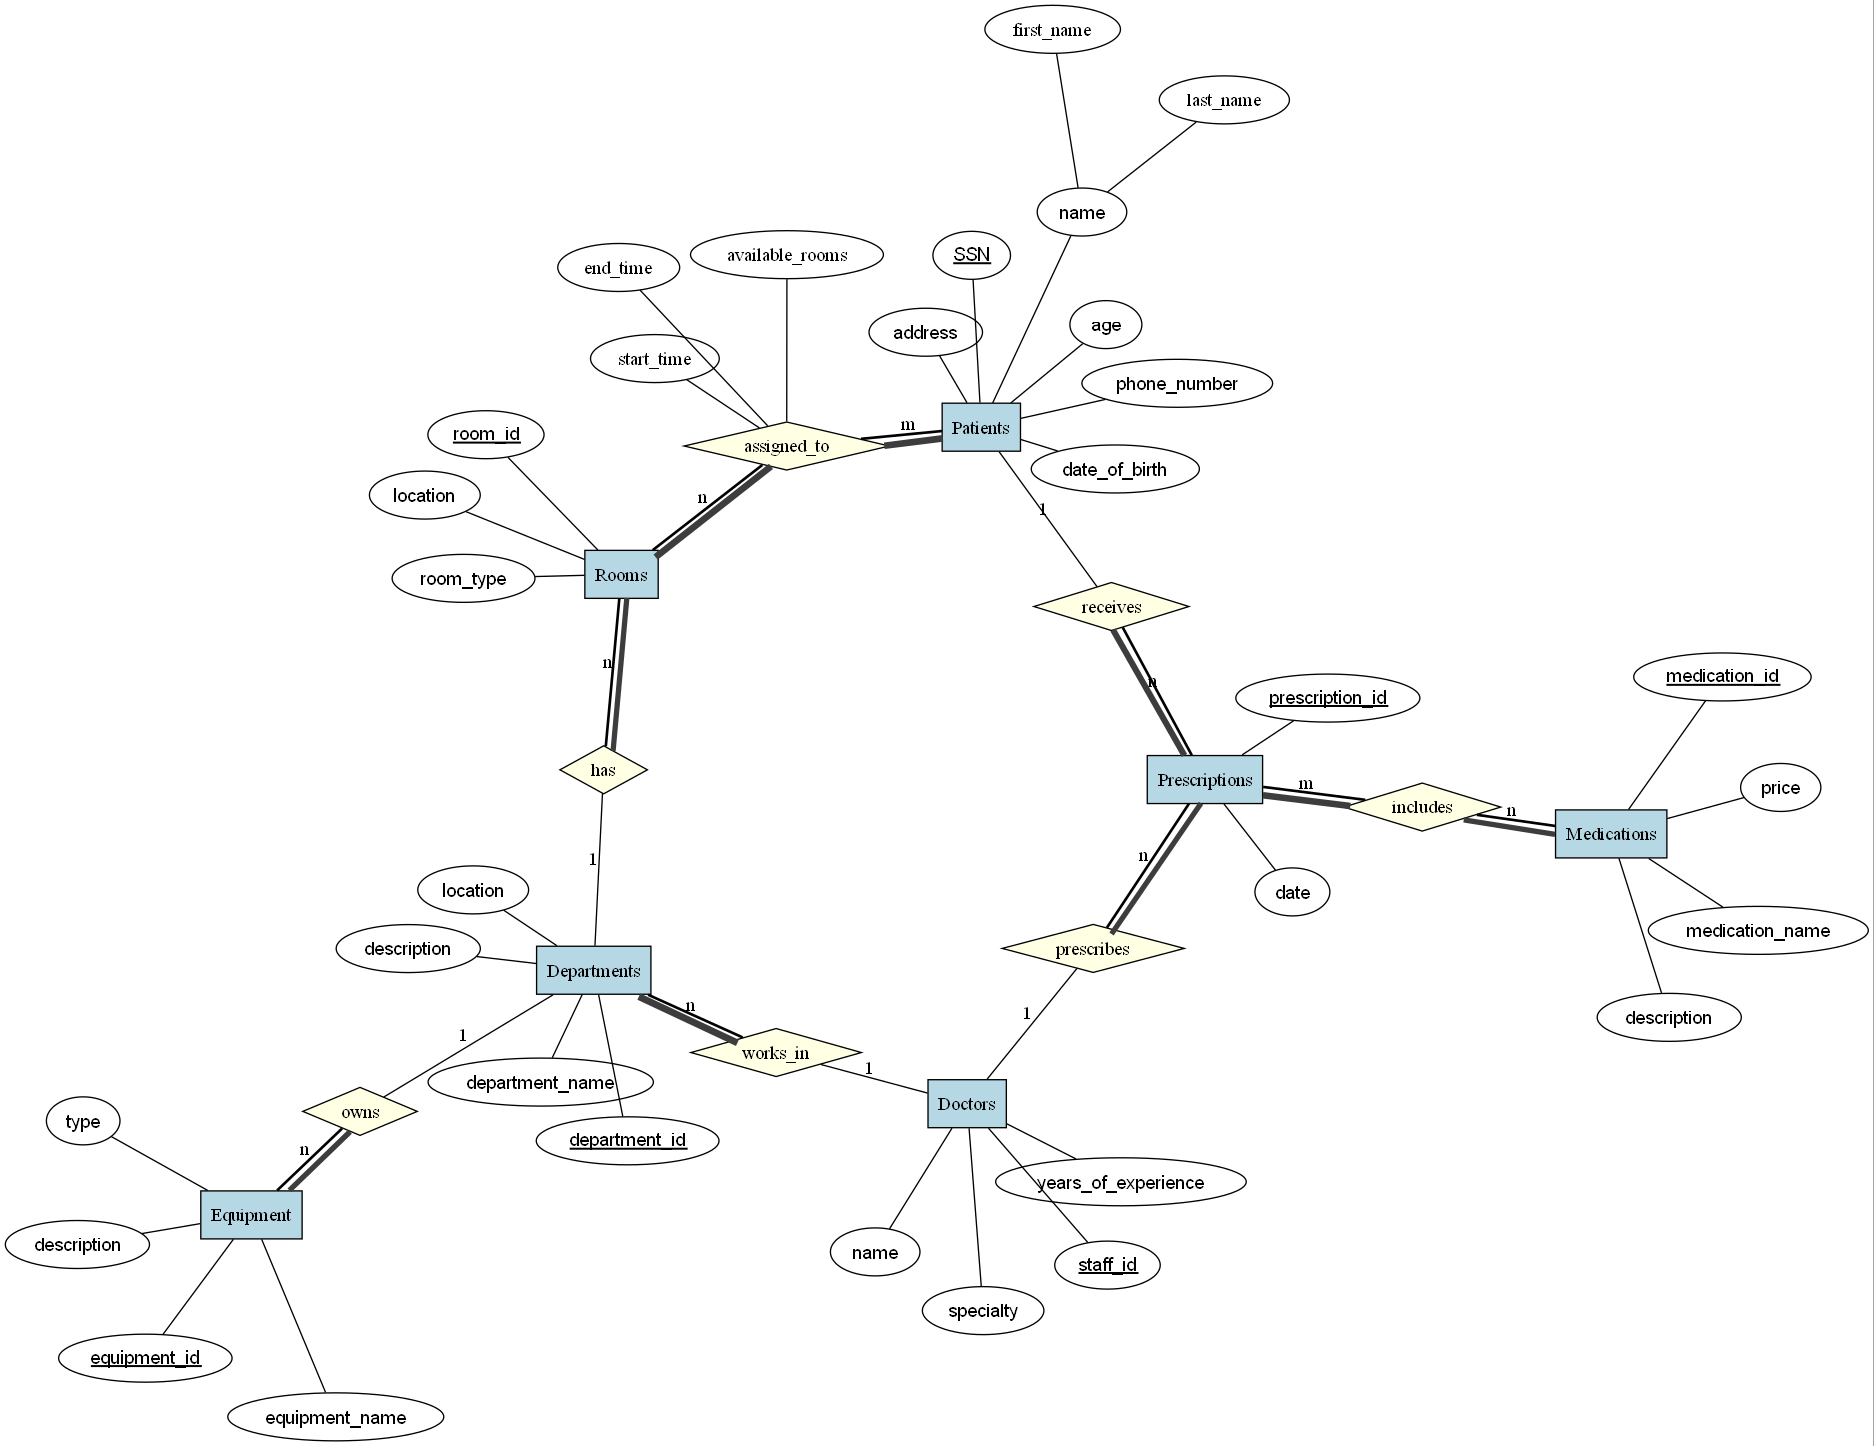
\includegraphics[width=1\linewidth]{Assignment1Q1.png}
    \caption{Assignment1Q1}
    \label{Assignment1Q1}
\end{figure}

The Python code for generating the diagram (since there is not double line in graphviz, I edited manually):

\begin{lstlisting}[language=Python, caption=Python code for generating the ER diagram]
from graphviz import Graph

def create_detailed_er_diagram():
    dot = Graph(comment='Detailed Hospital ER Diagram', engine='neato')
    dot.attr(rankdir='TB', size='200,200', overlap='false')

    # Entities
    entities = ['Doctors', 'Departments', 'Patients', 'Medications', 
                'Prescriptions', 'Rooms', 'Equipment']
    for entity in entities:
        dot.node(entity, entity, shape='box', style='filled', fillcolor='lightblue')

    # Attributes with underline for important ones
    attributes = {
        'Doctors': [('staff_id', True), ('name', False), ('specialty', False), 
                    ('years_of_experience', False)],
        'Departments': [('department_id', True), ('department_name', False), 
                        ('description', False), ('location', False)],
        'Patients': [('SSN', True), ('name', False), ('address', False), 
                     ('age', False), ('date_of_birth', False), 
                     ('phone_number', False)],
        'Medications': [('medication_id', True), ('medication_name', False), 
                        ('description', False), ('price', False)],
        'Prescriptions': [('prescription_id', True), ('date', False)],
        'Rooms': [('room_id', True), ('location', False), ('room_type', False)],
        'Equipment': [('equipment_id', True), ('equipment_name', False), 
                      ('type', False), ('description', False)]
    }

    for entity, attrs in attributes.items():
        for attr, is_important in attrs:
            attr_name = f"{entity}_{attr}"
            label = f"<u>{attr}</u>" if is_important else attr
            dot.node(attr_name, f'<<font face="Arial">{label}</font>>', shape='ellipse')
            dot.edge(entity, attr_name, style='solid')

    # Special handling for patient's name
    dot.node('Patients_first_name', 'first_name', shape='ellipse')
    dot.node('Patients_last_name', 'last_name', shape='ellipse')
    dot.edge('Patients_name', 'Patients_first_name', style='solid')
    dot.edge('Patients_name', 'Patients_last_name', style='solid')

    # Relationships with double lines for 'n' cardinality
    relationships = [
        ('Doctors', 'Departments', 'works_in', '1', 'n'),
        ('Patients', 'Prescriptions', 'receives', '1', 'n'),
        ('Doctors', 'Prescriptions', 'prescribes', '1', 'n'),
        ('Prescriptions', 'Medications', 'includes', 'm', 'n'),
        ('Departments', 'Rooms', 'has', '1', 'n'),
        ('Patients', 'Rooms', 'assigned_to', 'm', 'n'),
        ('Departments', 'Equipment', 'owns', '1', 'n')
    ]

    for start, end, label, start_card, end_card in relationships:
        rel_name = f"{start}_{end}_{label}"
        dot.node(rel_name, label, shape='diamond', style='filled', fillcolor='lightyellow')
        
        # Use double lines for 'n' or 'm' cardinality
        start_style = 'setlinewidth(2)' if start_card in ['n', 'm'] else ''
        end_style = 'setlinewidth(2)' if end_card in ['n', 'm'] else ''
        
        dot.edge(start, rel_name, label=start_card, style=start_style)
        dot.edge(rel_name, end, label=end_card, style=end_style)

    # Special handling for 'assigned_to' relationship
    dot.node('assigned_to_details1', 'start_time', shape='ellipse')
    dot.edge('Patients_Rooms_assigned_to', 'assigned_to_details1', style='solid')
    dot.node('assigned_to_details2', 'end_time', shape='ellipse')
    dot.edge('Patients_Rooms_assigned_to', 'assigned_to_details2', style='solid')
    dot.node('assigned_to_details3', 'available_rooms', shape='ellipse')
    dot.edge('Patients_Rooms_assigned_to', 'assigned_to_details3', style='solid')

    return dot

# Generate and save the diagram
er_diagram = create_detailed_er_diagram()
er_diagram.render('hospital_er_diagram_detailed', format='png', cleanup=True)
print("Detailed ER diagram has been generated as 'hospital_er_diagram_detailed.png'")
\end{lstlisting}


\section*{Question 2}
The diagram is shown below:

\begin{figure}[h]
    \centering
    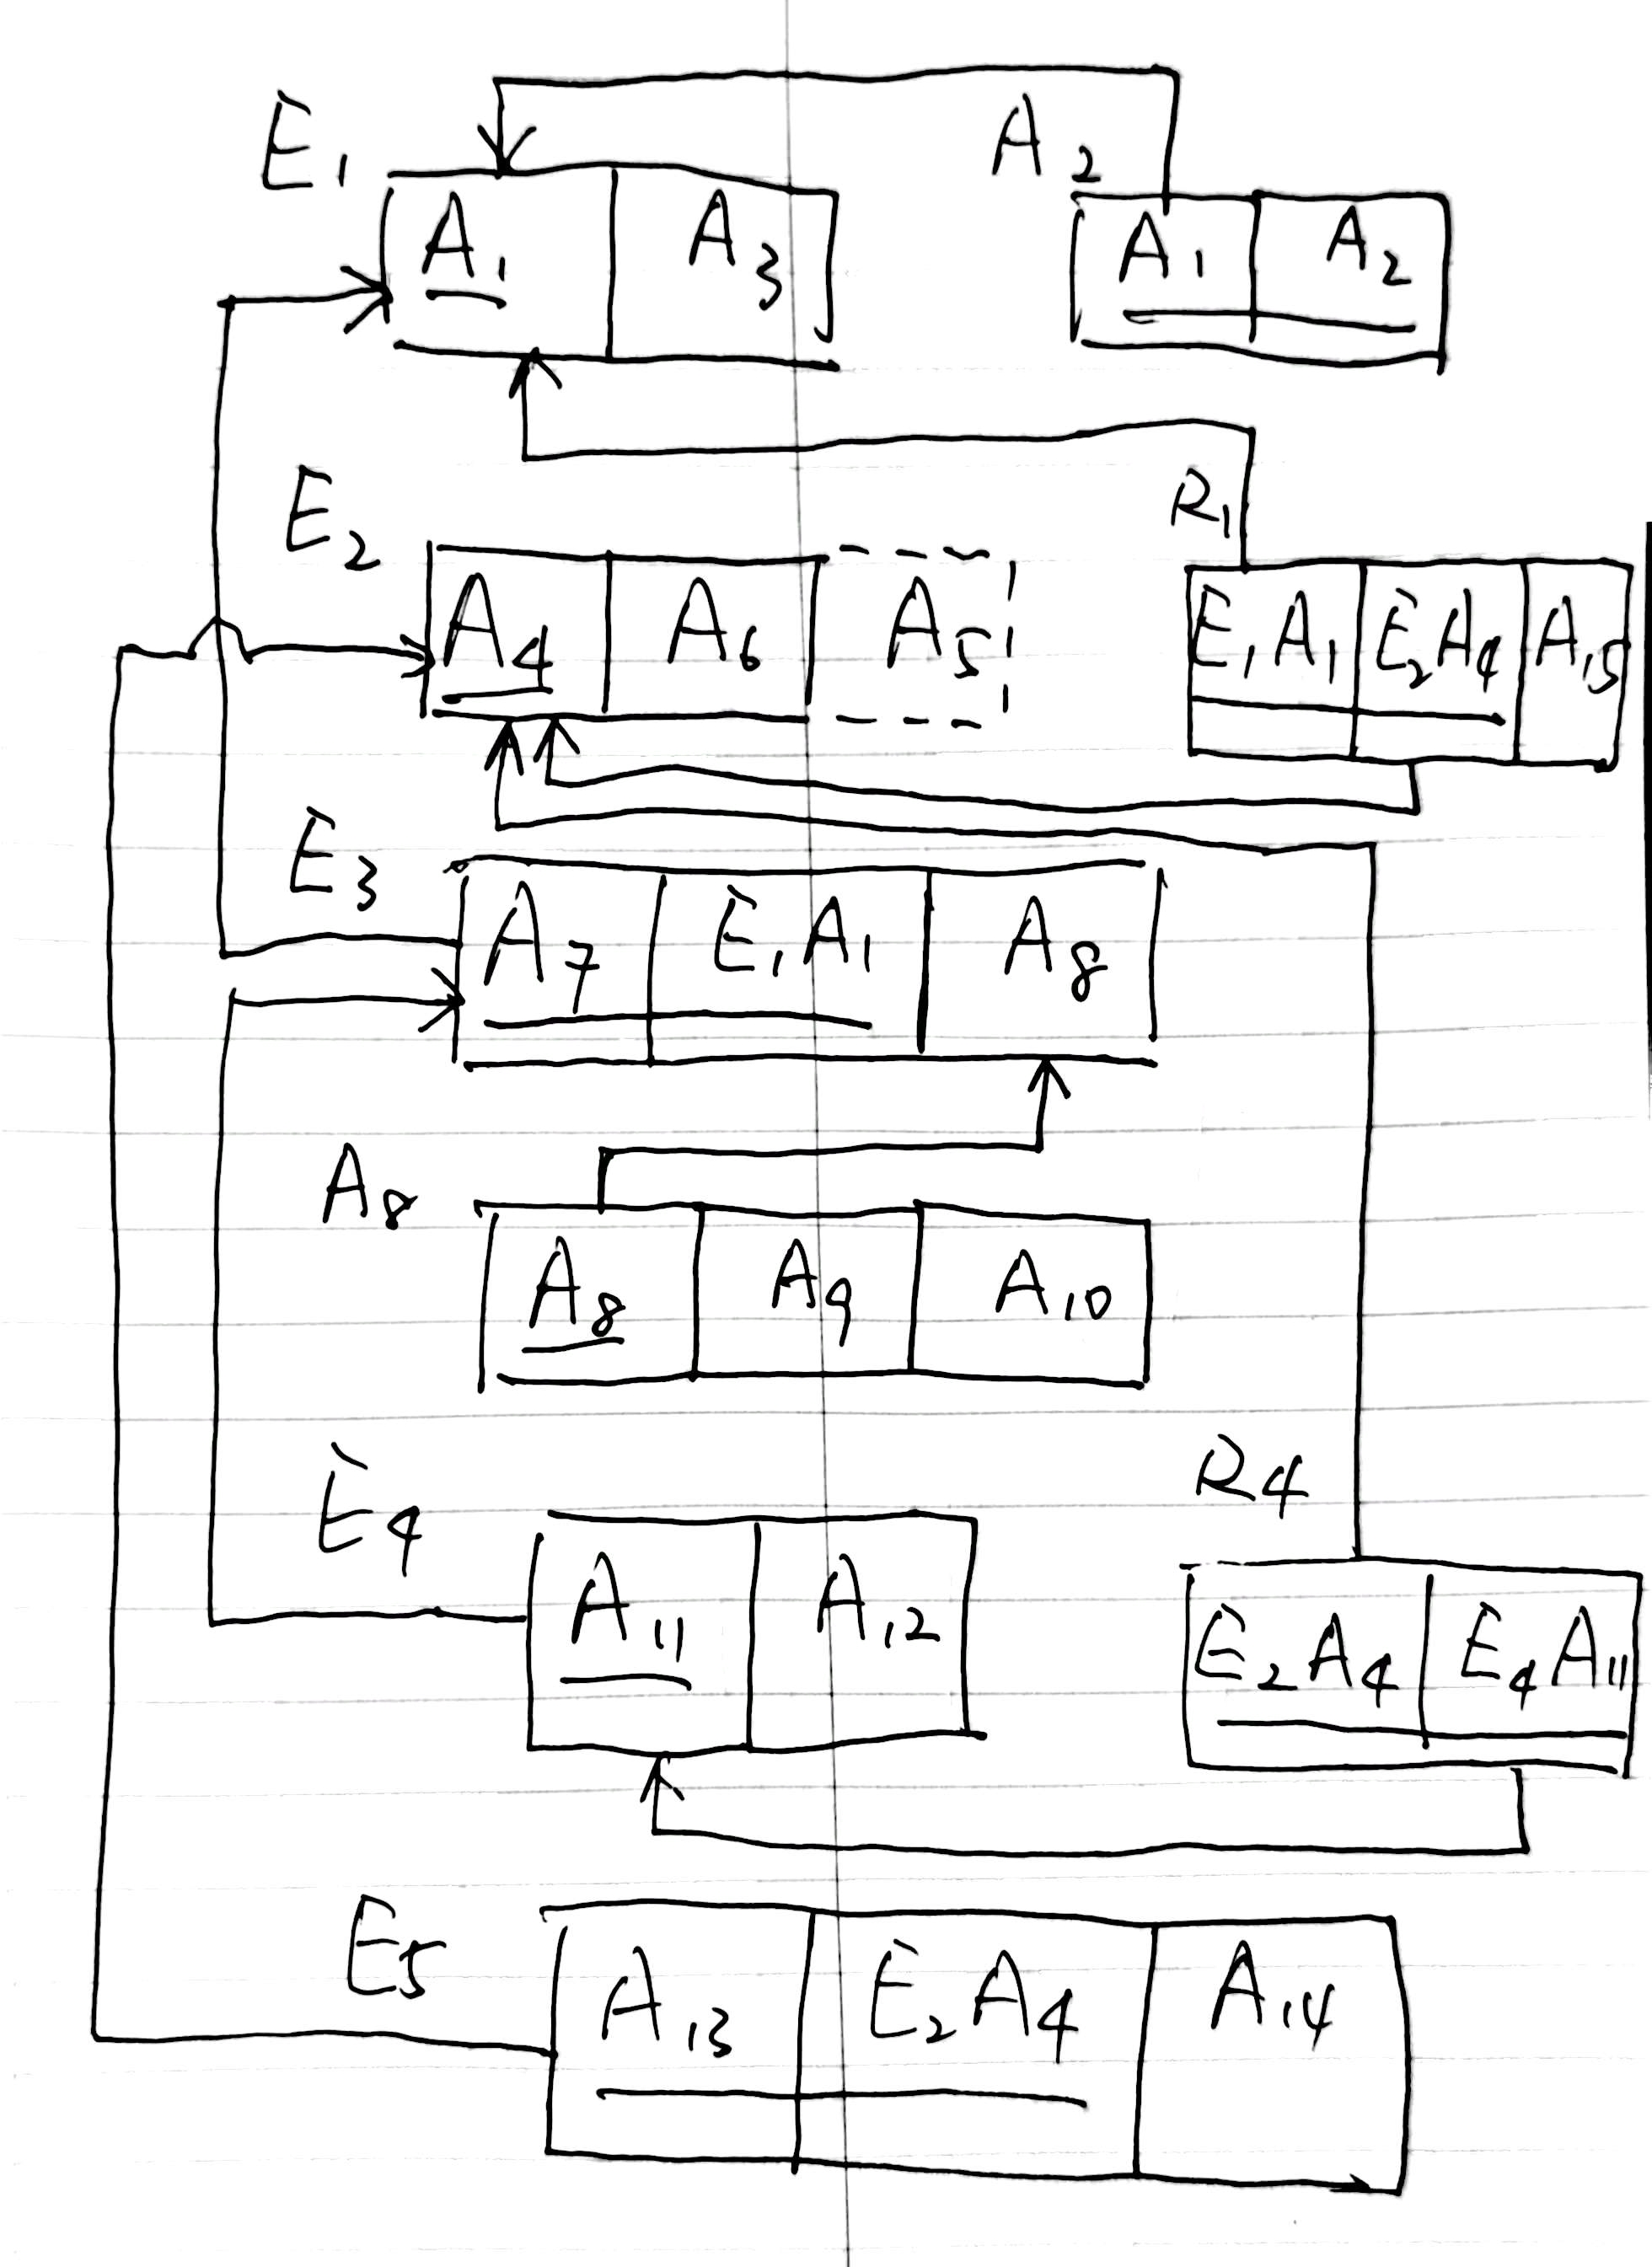
\includegraphics[width=0.5\linewidth]{Assignment1Q2.jpg}
    \caption{Assignment1Q2}
    \label{Assignment1Q2}
\end{figure}

\section*{Question 3}
Q1: 
\[
1.\ \text{TotalSpending}(\text{cusID}, \text{totalSpending}) \leftarrow \gamma_{\text{cusID}, \text{SUM}(\text{salePrice})} (\pi_{\text{cusID}, \text{salePrice}} (\text{Sale}))
\]
\[
2.\ \text{AvgSpending} \leftarrow \gamma_{\text{AVG}(\text{totalSpending})} (\text{TotalSpending})
\]
\[
3.\ \text{OverAvg}(\text{cusID}) \leftarrow \sigma_{\text{totalSpending} > \text{AvgSpending}} (\text{TotalSpending})
\]
\[
4.\ \text{CusNManu}(\text{cusID}, \text{manuCnt}) \leftarrow \gamma_{\text{cusID}, \text{COUNT}(\text{manuID})} (\text{Manufacturer} \bowtie \text{Car} \bowtie \text{Sale})
\]
\[
5.\ \text{MoreThan2}(\text{cusID}) \leftarrow \sigma_{\text{manuCnt} > 2} (\text{CusNManu})
\]
\[
6.\ \text{Result} \leftarrow \pi_{\text{cusName}} (\text{Customer} \bowtie_{\text{cusID}} (\text{OverAvg} \cap \text{MoreThan2}))
\]
\\
Q2: 
\[
1.\ \text{SerCnt}(\text{manuID}, \text{carID}, \text{sYear}, \text{serCnt}) \leftarrow \gamma_{\text{manuID}, \text{carID}, \text{sYear}, \text{COUNT}(\text{serID})} (\text{Manufacturer} \bowtie \text{Car} \bowtie \text{Service})
\]
\[
2.\ \text{LessThan1}(\text{manuID}, \text{carID}) \leftarrow \sigma_{\text{serCnt} \leq 1} (\text{SerCnt})
\]
\[
3.\ \text{MoreThan4\_5}(\text{manuID}) \leftarrow \sigma_{\text{rating} > 4.5} (\text{Manufacturer} \bowtie \text{Car} \bowtie \text{Sale} \bowtie \text{Salesperson})
\]
\[
4.\ \text{Result} \leftarrow \pi_{\text{manuID}} (\text{LessThan1}) \cap \pi_{\text{manuID}} (\text{MoreThan4\_5})
\]
\\
Q3: 
\[
1.\ \text{AvgPrice}(\text{saleYear}, \text{avgSalePrice}) \leftarrow \gamma_{\text{saleYear}, \text{AVG}(\text{salePrice})} (\pi_{\text{saleYear}, \text{salePrice}} (\text{Sale}))
\]
\[
2.\ \text{SalpNSale}(\text{salpID}, \text{salpName}, \text{saleYear}, \text{salePrice}) \leftarrow \pi_{\text{salpID}, \text{salpName}, \text{saleYear}, \text{salePrice}} (\text{Sale} \bowtie \text{Salesperson})
\]
\[
3.\ \text{SalpHigher}(\text{salpID}, \text{salpName}, \text{saleYear}) \leftarrow \pi_{\text{salpID}, \text{salpName}, \text{saleYear}} (\sigma_{\text{salePrice} > \text{avgSalePrice}} (\text{SalpNSale} \bowtie \text{AvgPrice}))
\]
\[
4.\ \text{SalesYear}(\text{salpID}, \text{salpName}, \text{minYear}, \text{maxYear}) \leftarrow \gamma_{\text{salpID}, \text{MIN}(\text{saleYear}), \text{MAX}(\text{saleYear})} (\text{SalpHigher})
\]
\[
5.\ \text{Result} \leftarrow \pi_{\text{salpName}} (\sigma_{\text{COUNT}(\text{saleYear}) = 2024 - \text{minYear}} (\gamma_{\text{salpName}, \text{minYear}, \text{COUNT}(\text{saleYear})} (\text{SalesYear})))
\]
\\
Q4: 
\[
1.\ \text{SerCnt}(\text{carID}, \text{serCount}) \leftarrow \gamma_{\text{carID}, \text{COUNT}(\text{serID})} (\text{Service})
\]
\[
2.\ \text{OneServiceCars}(\text{carID}) \leftarrow \sigma_{\text{serCount} = 1} (\text{SerCnt})
\]
\[
3.\ \text{ValidServiceCars}(\text{carID}) \leftarrow \sigma_{\text{sYear} \geq \text{saleYear} + 3} (\text{Sale} \bowtie \text{Service})
\]
\[
4.\ \text{Result} \leftarrow \text{OneServiceCars} \cap \text{ValidServiceCars}
\]


\end{document}
